\chapter{Co-simulation of power and ICT systems}
\label{ch:cosim}
\minitoc

\begin{tcolorbox}[width=\linewidth, sharp corners=all,
    colback=white!80!black,
    colframe=white!80!black]
This chapter is partly based on the following publication:
\begin{itemize}
    \item \fullcite{Cosim}
\end{itemize}
\end{tcolorbox}

As mentioned in appendix~\ref{ch:SPS}, a possible approach to model cyber-physical systems, i.e. system that consist of a ``physical'' part (in this case, a power grid) and a ``cyber'' part (i.e. ICT (information and communication technology) systems) that both act on each others, is through the use of co-simulations\footnote{Co-simulation can also refer to the simulation of part of a power system with RMS tools and part with EMT tools. This is however not the topic of this chapter.}. When performing co-simulations, both parts of the system are modelled using two separate simulators (e.g. \Dynawo{} for the physical part, and ns-3 for the cyber part) that are then run together. The advantage of co-simulation is that both parts can be easily modelled using dedicated simulators (with standard libraries, solvers, etc.), but the drawback is that additional work is needed to make the two simulators run together. Indeed, the two simulators need to stay synchronised and exchange information about what is currently happening in both simulators (in order to model the interactions between the cyber and physical parts).

Before talking about time synchronisation of simulators, it can be noted that ICT and power system simulators have a different concept of time. Indeed, power system simulators work by solving a set of differential-algebraic equations (DAEs) that model the behaviour of the grid. Time is thus seen as a continuous variable (as the grid continuously evolves), although when numerically solving the DAEs, time will be discretised using a fixed or variable time step. On the other hand, ICT simulators are ``event-based'' which means that the state of the system only changes following events, and \emph{nothing} occurs in between.

To illustrate this, let's consider a very simple ICT system consisting of two nodes sending a message back-and-forth between each other through a communication link that has a 10ms propagation delay. Let's assume that the simulation starts with node 1 sending the message to node 2 at \(t=0ms\). At the start of the simulation, the event queue of the simulator thus contains a single event ``Node 1 sends a message at \(t=0ms\)''. The simulator then simulates this event, removes it from the queue, and creates a new event ``Node 2 receives a message at \(t=10ms\)''. The simulator then proceeds to this new event, removes it from the queue and creates a third event ``Node 2 sends a message at \(t=10ms\)''. The simulator continues like this until the event queue is empty or until \(t\) reaches the maximum simulation time.

Due to these differences between physical and cyber simulators, multiple approaches have been defined to synchronise them as discussed in~\cite{CosimFigure}. The most common approaches are illustrated in Figure~\ref{fig:Cosim}. The most straightforward approach consists in synchronising the simulators at predefined time intervals as shown in Figure~\ref{fig:CosimPointBased} and is referred to as point-based synchronisation. In other words, each time a simulator reaches a synchronisation point, it waits for the other simulator to also reach this point, then the two simulators exchange data about what occurred since the last synchronisation, and go back to simulating separately until the next synchronisation point. The drawback of this method is that when something happens in a simulator, the other is not made aware of it until the next synchronisation step. Events are thus perceived as ``delayed'' by the other simulator.

\begin{figure}
\centering
\subfloat[Point-based synchronisation]{%
\label{fig:CosimPointBased}
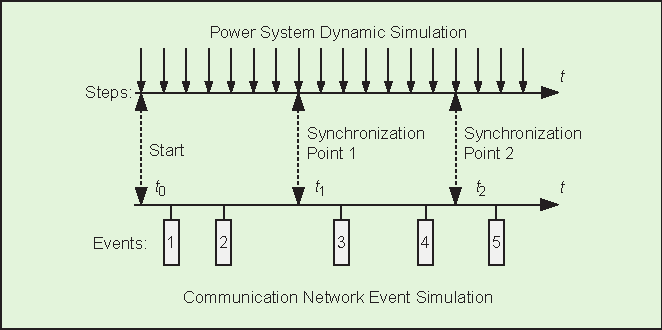
\includegraphics[width=0.7\linewidth]{Figs/CosimPointBased.pdf}
} \\ \vspace*{0.5cm} % \hfill
\subfloat[Event-based synchronisation]{%
\label{fig:CosimEventBased}
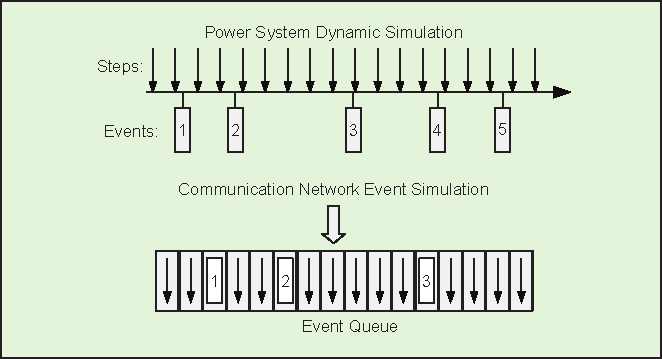
\includegraphics[width=0.7\linewidth]{Figs/CosimEventBased.pdf}
}
\caption{Main synchronisation techniques for co-simulation of cyber-physical systems~\cite{CosimFigure}}
\label{fig:Cosim}
\end{figure}

The second most common approach is the event-based synchronisation method illustrated in Figure~\ref{fig:CosimEventBased}. In this approach, time steps of the power system simulators and events in the cyber simulator are merged in a global event queue and the simulators are synchronised at each step of the global event queue (i.e. at each time step of the power system simulator, and for each event in the cyber simulator). The advantage of this method is that simulators are directly made aware when something occurs in the second simulator. It has however two important drawbacks. The first is that it is difficult to implement for power system simulators with variable integration time steps. Indeed, such simulators cannot say in advance what will be their next time step as it depends on zero-crossings and on numerical convergence. So complex rollback mechanisms must be implemented to account for cases where the power system simulator time step is smaller than predicted.

The second important drawback is that ICT simulators tend to generate events at a very fast rate (sub-millisecond rate or even lower) compared to the timescales of interest in power systems. Consider for example the test case shown in Figure~\ref{fig:IEEE_PMU} consisting of the standard IEEE 39-bus test system but equipped with a phasor measurement unit (PMU)-based state estimator. In this system, PMUs are installed at each bus and send measurements to phasor data concentrators (PDCs) every 30 times per second (the IEEE 39-bus system is US-based and is thus considered to be operated at 60~Hz in this chapter). PDCs aggregate this data and forward it to a super PDC (SPDC) that perform the state estimation and potentially initiate automatic corrective actions based on the state of the system.

\begin{figure}
\centering
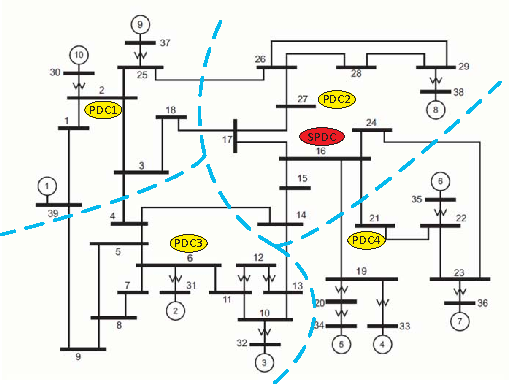
\includegraphics[width=0.6\linewidth]{Figs/IEEE39-PMU.pdf}
\caption{IEEE 39-bus test system with an all-PMU state estimator~\cite{GECOtestcase}}
\label{fig:IEEE_PMU}
\end{figure}

In this case, there are 39 PMUs that send messages to the communication network 30 times per second. If we take as a rough estimate that there are in average 3 hops between a PMU and the SPDC, this results in 3500 events and thus 3500 synchronisation steps per second, or in average, a synchronisation step every 0.3ms. Synchronisation steps would be even more frequent for larger systems. However, there is no point to have such frequent synchronisations as power system dynamics (at least the ones considered when using RMS simulators) are significantly slower.

The point-based synchronisation technique should thus be used in the majority of cases. For this approach, Table~\ref{tab:CosimComputationTime} analyses the impact of the co-simulation time step (i.e. how often the simulators are synchronised) on the total computation time for the above test case. The computation time is 4s when using a very large co-simulation time step (5000ms, effectively never synchronising the two simulators) and 16s, four times more, when using a very small step of 1ms. And actually, this increase in computation time is mostly due to the fact that a smaller co-simulation time step forces the power system simulator to use a smaller integration time step (the power system cannot use a 1s integration time step if synchronisations are performed every millisecond). Computations have been performed using a standard laptop CPU (AMD 4500U) and are significantly faster than the 20~minutes taken for a similar system in~\cite{GECOcomputationTime}. The reason for this is simply due to a better implementation. In~\cite{GECOcomputationTime}, authors use a closed-source power system simulator that does not have an interface designed to be used in a co-simulation. They are thus probably forced to stop the simulator, write power system to a file to disk, then to read this file and send the necessary values to the cyber simulator at each synchronisation time step. Our implementation connects \Dynawo{} and ns-3 using HELICS~\cite{HELICS}, a co-simulation orchestrator that enables efficient data exchanges through RAM, and is thus significantly faster.

\begin{table}
\centering
\caption{Evolution of computation time with using self-consistent and co-simulation. The simulated time is 5s.}
\begin{tabular}{@{}ll@{}}
\toprule
Co-simulation time step (ms) & Computation time \\ \midrule
5000ms                       & 4s               \\
10ms                         & 7s               \\
1ms                          & 16s              \\ \bottomrule
\end{tabular}
\label{tab:CosimComputationTime}
\end{table}
